\documentclass[tikz,border=12pt]{standalone}
\usepackage{tikz}
\usepackage{amsmath,amssymb}
\usetikzlibrary{arrows.meta, calc, positioning}

% ---- colours ----
\definecolor{cBlue}{RGB}{13,110,200}
\definecolor{cGray}{RGB}{95,108,120}
\definecolor{cOrange}{RGB}{195,95,15}
\definecolor{cFillBlue}{RGB}{230,242,255}
\definecolor{cFillGray}{RGB}{237,239,242}
\definecolor{cFillOrange}{RGB}{255,239,218}
\definecolor{cRed}{RGB}{170,35,35}
\definecolor{cGreen}{RGB}{30,145,75}
\definecolor{cLegend}{RGB}{250,251,253}

\tikzset{
  nd/.style={circle, draw, minimum size=2.6cm, align=center,
             font=\bfseries\small, inner sep=2pt, line width=1.6pt},
  nBlue/.style  ={nd, draw=cBlue,   fill=cFillBlue,   text=cBlue},
  nGray/.style  ={nd, draw=cGray,   fill=cFillGray,   text=cGray},
  nOrange/.style={nd, draw=cOrange, fill=cFillOrange, text=cOrange, dashed},
  myarr/.style={->,>=Stealth, line width=1.35pt, font=\scriptsize, align=center},
  aBlue/.style  ={myarr, color=cBlue},
  aRed/.style   ={myarr, color=cRed},
  aGreen/.style ={myarr, color=cGreen},
  aOrange/.style={myarr, color=cOrange},
}

\begin{document}
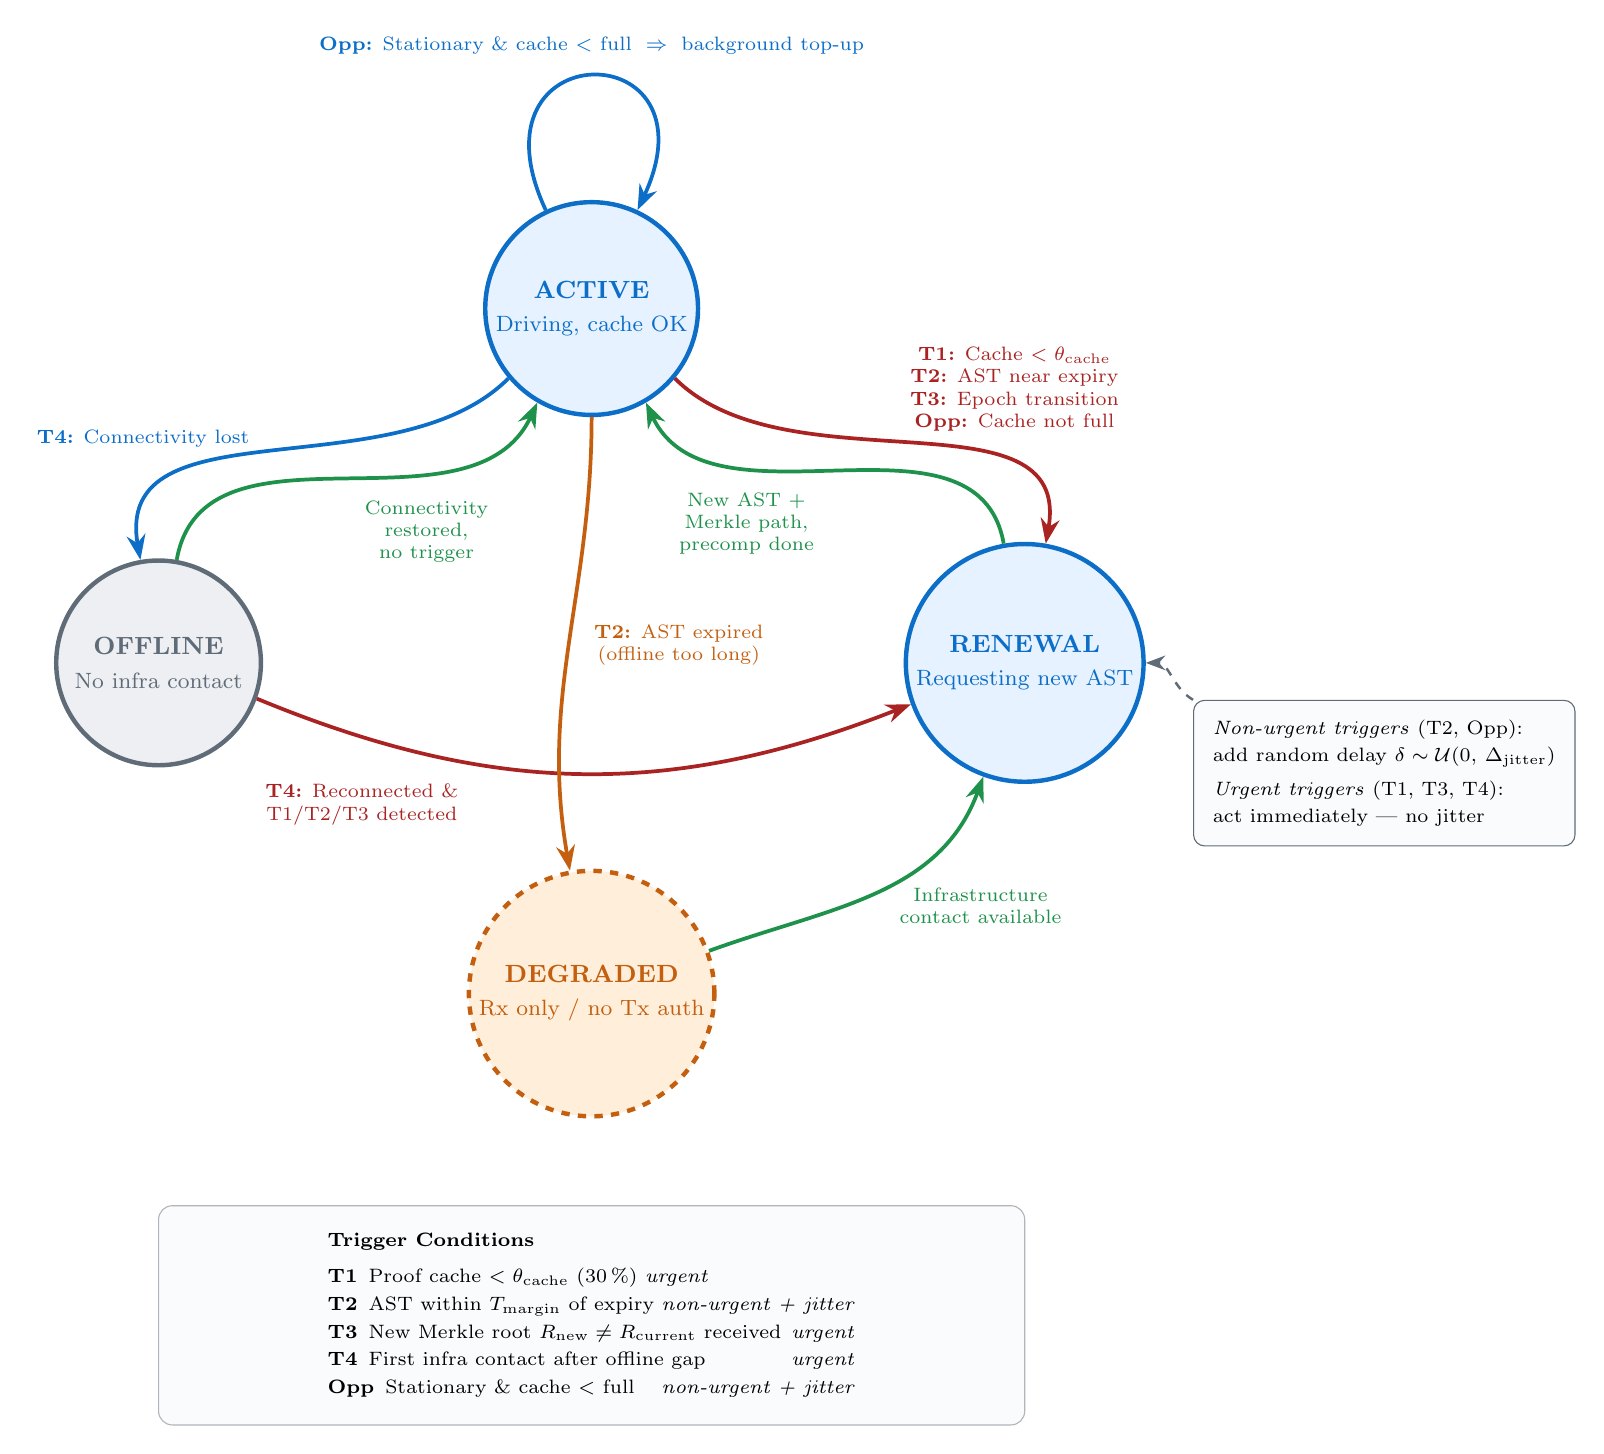
\begin{tikzpicture}

%% ============================================================
%% STATE NODES  -- triangular arrangement
%%   ACTIVE   : top-centre
%%   OFFLINE  : bottom-left
%%   RENEWAL  : bottom-right
%%   DEGRADED : below ACTIVE (dangles down from centre)
%% ============================================================
\node[nBlue]   (active)   at ( 0.0,  4.5) {ACTIVE\\[1pt]%
  {\footnotesize\mdseries Driving, cache OK}};

\node[nGray]   (offline)  at (-5.5,  0.0) {OFFLINE\\[1pt]%
  {\footnotesize\mdseries No infra contact}};

\node[nBlue]   (renewal)  at ( 5.5,  0.0) {RENEWAL\\[1pt]%
  {\footnotesize\mdseries Requesting new AST}};

\node[nOrange] (degraded) at ( 0.0, -4.2) {DEGRADED\\[1pt]%
  {\footnotesize\mdseries Rx only / no Tx auth}};

%% ============================================================
%% ACTIVE  <-->  OFFLINE
%% ============================================================
% Active -> Offline  (left side, going down-left)
\draw[aBlue]
  (active.220) to[out=225, in=100]
  node[left, midway, xshift=-4pt, yshift=5pt]
    {\textbf{T4:} Connectivity lost}
  (offline.100);

% Offline -> Active  (right side, going up-right)
\draw[aGreen]
  (offline.80) to[out=80, in=245]
  node[right, midway, xshift=4pt, yshift=-20pt]
    {Connectivity\\restored,\\no trigger}
  (active.240);

%% ============================================================
%% ACTIVE  <-->  RENEWAL
%% ============================================================
% Active -> Renewal  (right side, going down-right)
\draw[aRed]
  (active.320) to[out=315, in=80]
  node[right, midway, xshift=-5pt, yshift=20pt]
    {\textbf{T1:} Cache $<\theta_{\text{cache}}$\\
     \textbf{T2:} AST near expiry\\
     \textbf{T3:} Epoch transition\\
     \textbf{Opp:} Cache not full}
  (renewal.80);

% Renewal -> Active  (left side, going up-left)
\draw[aGreen]
  (renewal.100) to[out=100, in=295]
  node[left, midway, xshift=-5pt, yshift=-20pt]
    {New AST +\\Merkle path,\\precomp done}
  (active.300);

%% ============================================================
%% OFFLINE  <-->  RENEWAL  (bottom arc)
%% ============================================================
\draw[aRed, bend right=22]
  (offline.340) to
  node[below, midway, xshift=-80pt]
    {\textbf{T4:} Reconnected \& \\ T1/T2/T3 detected}
  (renewal.200);

%% ============================================================
%% ACTIVE  -->  DEGRADED
%% ============================================================
\draw[aOrange]
  (active.270) to[out=270, in=100]
  node[right, midway, xshift=5pt]
    {\textbf{T2:} AST expired\\(offline too long)}
  (degraded.100);

%% ============================================================
%% DEGRADED  -->  RENEWAL
%% ============================================================
\draw[aGreen]
  (degraded.20) to[out=20, in=250]
  node[right, midway, xshift=5pt, yshift=-5pt]
    {Infrastructure\\contact available}
  (renewal.250);

%% ============================================================
%% ACTIVE self-loop  (opportunistic)
%% ============================================================
\draw[aBlue]
  (active) edge[loop above, looseness=5.5, out=115, in=65]
  node[above, yshift=4pt]
    {\textbf{Opp:} Stationary \& cache $<$ full $\;\Rightarrow\;$ background top-up}
  (active);

%% ============================================================
%% JITTER ANNOTATION  (bottom-right)
%% ============================================================
\node[
  draw=cGray, rounded corners=4pt, fill=cLegend,
  font=\scriptsize, align=left, inner sep=7pt,
  right=0.6cm of renewal, yshift=-1.4cm
] (jitter) {
  \textit{Non-urgent triggers} (T2, Opp):\\[2pt]
  add random delay $\delta\sim\mathcal{U}(0,\,\Delta_{\text{jitter}})$\\[4pt]
  \textit{Urgent triggers} (T1, T3, T4):\\[2pt]
  act immediately --- no jitter
};
\draw[->,>=Stealth, dashed, cGray, line width=0.9pt]
  (jitter.north west) to[out=150,in=0] (renewal.east);

%% ============================================================
%% LEGEND  (bottom strip)
%% ============================================================
\node[
  draw=cGray!50, rounded corners=5pt, fill=cLegend,
  inner sep=10pt, below=1.1cm of degraded,
  font=\scriptsize, align=left, minimum width=11cm
] {
  \textbf{Trigger Conditions}\\[5pt]
  \textbf{T1}\enspace Proof cache $<\theta_{\text{cache}}$ (30\,\%)
    \hfill\textit{urgent}\\[2pt]
  \textbf{T2}\enspace AST within $T_{\text{margin}}$ of expiry
    \hfill\textit{non-urgent + jitter}\\[2pt]
  \textbf{T3}\enspace New Merkle root $R_{\text{new}}\neq R_{\text{current}}$ received
    \hfill\textit{urgent}\\[2pt]
  \textbf{T4}\enspace First infra contact after offline gap
    \hfill\textit{urgent}\\[2pt]
  \textbf{Opp}\enspace Stationary \& cache $<$ full
    \hfill\textit{non-urgent + jitter}
};

\end{tikzpicture}
\end{document}